% !TEX root = ../main.tex
% chktex-file 46
\chapter{Related Work}%
\label{sec:related}

Before combining \ac{lta} and \ac{gcr} as described in \cref{sec:intro:goals}, we first give an overview of the state-of-the-art in both fields of research.
This is done in three steps:
\begin{enumerate}
	\item We begin with an overview of the existing \ac{lta} methods for unstructured inputs.
	\item Then we look at the domain of structured inputs.
		To solve the \ac{gcr} problem, relevant graphs characteristics have to be defined in order to determine the similarity and dissimilarity of graphs.
		We will look at two common approaches for graph characterization: The \acl{wl} algorithm and the notion of graph spectra.
	\item Using the described graph characterization approaches, a brief overview of current \ac{gcr} methods will then be given.
\end{enumerate}

\section{Learning to Aggregate}%
\label{sec:related:lta}

The class of \ac{lta} problems was first described by \citet{Melnikov2016}.
There an input instance is understood as a composition $\bm{c} = \ldblbrace c_1, \dots, c_n \rdblbrace$ of so-called constituents, i.e.\ as a variable-size multiset (denoted as $\ldblbrace \cdot \rdblbrace$).
The assumption in \ac{lta} problems is that for all constituents $c_i \in \bm{c}$ a local score $y_i \in \mathcal{Y}$ is either given or computable.
The set of those local scores should be indicative of the overall score $y \in \mathcal{Y}$ of the composition $\bm{c}$.
\ac{lta} problems typically require two subproblems to be solved:
\begin{enumerate}[label=\textbf{\arabic*.}]
	\item \textbf{Aggregation:}
		A variadic aggregation function $\mathcal{A}: \mathcal{Y}^{*} \to \mathcal{Y}$ that estimates composite scores has to be learned, i.e.\@ $y_i \approx \hat{y} = \mathcal{A}(y_{1}, \dots, y_{n})$.
		Typically the aggregation function $\mathcal{A}$ should be associative and commutative to fit with the multiset-structure of compositions.
	\item \textbf{Disaggregation:}
		In case the constituent scores $y_i$ are not given, they have to be derived from a constituent representation, e.g.\ a vector $x_i \in \mathcal{X}$.
		To learn this derivation function $f: \mathcal{X} \to \mathcal{Y}$, only the constituent vectors ${\ldblbrace x_i \rdblbrace}_{i = 1}^{n}$ and the composite score $y$ is given.
		Thus the constituent scores $y_i$ need to be \textit{disaggregated} from $y$ in order to learn $f$.
\end{enumerate}
\begin{figure}[ht]
	\centering
	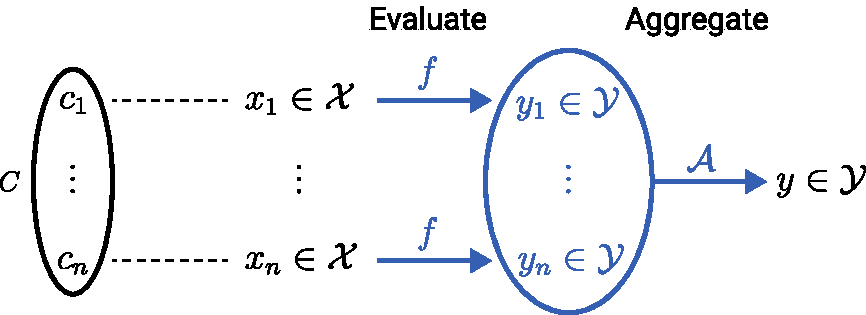
\includegraphics[width=0.7\linewidth]{gfx/related-work/lta-overview.pdf}
	\caption{Overview of the structure of LTA for multiset compositions.}\label{fig:related:lta-overview}
\end{figure}
Overall \ac{lta} can be understood as the joint problem of learning the aggregation function $\mathcal{A}$ and the local score derivation function $f$.
Two main approaches to represent the aggregation function in \ac{lta} problems have been explored.

\subsection{Uninorm-Aggregation}%
\label{sec:related:lta:uninorm}

The first approach uses \textit{uninorms}~\cite{Melnikov2016} to do so.
There the basic idea is to express composite scores as fuzzy truth assignments $y \in [0, 1]$.
Such a composite assignment $y$ is modeled as the result of a parameterized logical expression of constituent assignments $y_i \in [0, 1]$.
As the logical expression that thus effectively aggregates the constituents, a uninorm $U_{\lambda}$ is used.
Depending on the parameter $\lambda \in [0, 1]$, $U_{\lambda}$ combines a t-norm $T$ and a t-conorm $S$ which are continuous generalizations of logical conjunction and disjunction respectively.
One popular choice of norms are the so-called Łukasiewicz norms:
\begin{align}
	\text{t-norm } T(a, b) &:= \max \{ 0, a + b - 1 \}, \quad\text{t-conorm } S(a, b) := \min \{ a + b, 1 \}, \nonumber \\
	\text{uninorm } U_\lambda(a, b) &:= \begin{cases}
		\lambda T\left(\frac{a}{\lambda}, \frac{b}{\lambda}\right) & \text{if } a, b \in [0, \lambda] \\
		\lambda + (1 - \lambda) S\left(\frac{a - \lambda}{1 - \lambda}, \frac{b - \lambda}{1 - \lambda}\right) & \text{if } a, b \in [\lambda, 1] \\
		\lambda \min \{ a, b \} & \text{else}
	\end{cases}
\end{align}
At the extreme points $(0, 0)$, $(0, 1)$, $(1, 0)$ and $(1, 1)$, $T$ and $S$ coincide with the Boolean operators $\land$ and $\lor$;
the values at all other points are interpolated as shown in \cref{fig:related:logic-norms}.
The uninorm $U_\lambda$ uses the conjunctive t-norm $T$ for values below the threshold $\lambda$ and the disjunctive t-conorm $S$ for values above the threshold.
$U_\lambda$ therefore smoothly interpolates between a conjunctive and disjunctive operator with the extreme points $U_1 = T$ and $U_0 = S$.
\begin{figure}[ht]
	\centering
	\begin{tikzpicture}
		\begin{axis}[
			title={t-norm $T$ ($\land$)},
			xlabel=$a$,
			ylabel=$b$,
			xlabel style={xshift=0.2cm, yshift=0.15cm},
			ylabel style={xshift=-0.2cm, yshift=0.15cm},
			tick label style={font=\scriptsize},
			width=0.33\textwidth,
			colormap = {bluered}{color(0cm) = (t_blue); color(1cm) = (t_red)}
		]
			\addplot3[
				mesh,
				samples=12,
				domain=0:1,
				domain y=0:1
			]{max(x + y - 1, 0)};
		\end{axis}
	\end{tikzpicture}
	\begin{tikzpicture}
		\begin{axis}[
			title={t-conorm $S$ ($\lor$)},
			xlabel=$a$,
			ylabel=$b$,
			xlabel style={xshift=0.2cm, yshift=0.15cm},
			ylabel style={xshift=-0.2cm, yshift=0.15cm},
			tick label style={font=\scriptsize},
			width=0.33\textwidth,
			colormap = {bluered}{color(0cm) = (t_blue); color(1cm) = (t_red)}
		]
			\addplot3[
				mesh,
				samples=12,
				domain=0:1,
				domain y=0:1
			]{min(x + y, 1)};
		\end{axis}
	\end{tikzpicture}
	\begin{tikzpicture}
		\begin{axis}[
			title={uninorm $U_{0.5}$ ($\land$/$\lor$)},
			xlabel=$a$,
			ylabel=$b$,
			xlabel style={xshift=0.2cm, yshift=0.15cm},
			ylabel style={xshift=-0.2cm, yshift=0.15cm},
			tick label style={font=\scriptsize},
			width=0.33\textwidth,
			colormap = {bluered}{color(0cm) = (t_blue); color(1cm) = (t_red)}
		]
			\addplot3[
				mesh,
				samples=12,
				domain=0:1,
				domain y=0:1
			]{(x <= 0.5 && y <= 0.5) * 0.5 * max(2 * (x + y) - 1, 0) + (x > 0.5 && y > 0.5) * (0.5 + 0.5 * min(2 * (x + y - 1), 1)) + (!(x <= 0.5 && y <= 0.5) && !(x > 0.5 && y > 0.5)) * min(x, y)};
		\end{axis}
	\end{tikzpicture}
	\caption{The Łukasiewicz norms and the corresponding uninorm for $\lambda = 0.5$.}\label{fig:related:logic-norms}
\end{figure}

Since t-norms and t-conorms are commutative and associative they can also be applied to non-empty sets of arbitrary size, i.e. $T(\ldblbrace y_1, \dots, y_n \rdblbrace) = T(y_1, T(\ldblbrace y_2, \dots, y_n \rdblbrace))$ with fixpoint $T(\ldblbrace y \rdblbrace) = y$.
Using this extension, a uninorm $U_\lambda$ can be applied to sets which turns it into a parameterized aggregation function $\mathcal{A}_\lambda: {[0, 1]}^* \to [0, 1]$.
In this simple model the \ac{lta} aggregation problem boils down to the optimization of $\lambda$.
The \ac{lta} disaggregation problem is solved by jointly optimizing a \acf{lm}, i.e.\ the constituent scores ${\ldblbrace y_i \in [0, 1] \rdblbrace}_{c_i \in \bm{c}}$ are described by $y_i = {\left( 1 + \exp(-\theta^\top x_i) \right)}^{-1}$.
Overall an \ac{lta} model is therefore described by the uninorm parameter $\lambda$ and the regression coefficients $\theta$.

\subsection{\acs*{owa}-Aggregation}%
\label{sec:related:lta:owa}

Recently \citet{Melnikov2019} have looked at an alternative class of aggregation functions.
Instead of using fuzzy logic to describe score aggregation, \ac{owa} operators were used.
\ac{owa} aggregators work by sorting the input scores and then weighting them based on their sort position, i.e.\ %
\begin{align}
	\mathcal{A}_{\lambda}(y_1, \dots, y_n) := \sum_{i = 1}^n \lambda_i y_{\pi(i)},
\end{align}
where $\lambda \in \mathbb{R}^n$ is a weight vector with ${\|\lambda\|}_1 = 1$ and $\pi$ is a sorting permutation of the input scores with $y_i < y_j \Rightarrow \pi(i) < \pi(j)$. % chktex 21
Depending on the choice of the vector $\lambda$, the \ac{owa} function $\mathcal{A}_\lambda$ can express common aggregation functions like
$\min$ (if $\lambda = (1, 0, \dots, 0)$),
$\max$ (if $\lambda = (0, \dots, 0, 1)$)
or the arithmetic mean (if $\lambda = \left(\frac{1}{n}, \dots, \frac{1}{n}\right)$).

To deal with varying composition sizes $n$, the weights $\lambda_1, \dots, \lambda_n$ can however not be statically assigned.
Instead they are interpolated using a so-called \ac{bum} function $q: [0, 1] \to [0, 1]$.
It takes constituent positions that are normalized to the unit interval, i.e.\ $\frac{i}{n} \in [0, 1]$.
The \ac{bum} function $q$ is then used to interpolate a weight for any normalized sort position via $\lambda_i := q\left(\frac{i}{n}\right) - q\left(\frac{i - 1}{n}\right)$.
Because $q$ is monotone with $q(0) = 0$ and $q(1) = 1$, it always holds that ${\|\lambda\|}_1 = q(1) - q(0) = 1$. % chktex 21
Using this model, the aggregation problem boils down to optimizing the shape of $q$.

\begin{figure}[ht]
	\centering
	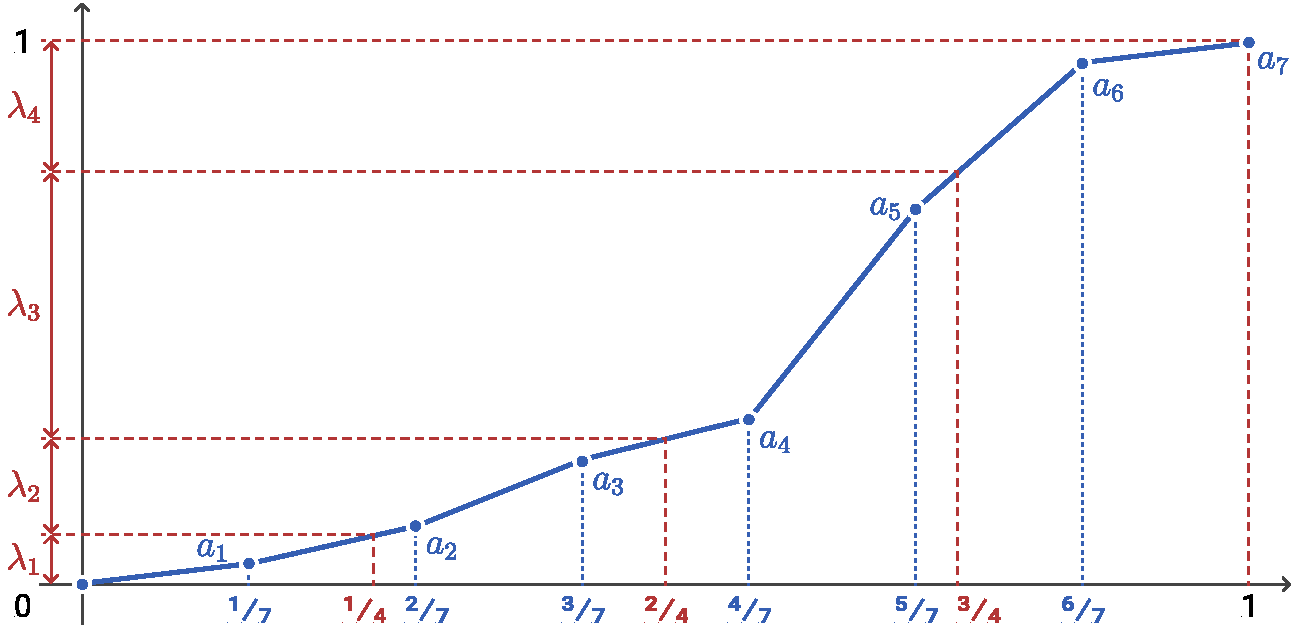
\includegraphics[width=0.75\linewidth]{gfx/related-work/bum.pdf}
	\caption[Illustration of how a \ac{bum} function is described as a linear spline and its relation to the \ac{owa} weights.]{
		Illustration of how \textcolor{t_blue}{$a$} describes \textcolor{t_blue}{$q$} and its relation to \textcolor{t_red}{$\lambda$} ($n = 4$, $m = 7$).
	}\label{fig:related:bum}
\end{figure}
In the \ac{owa} approach the \ac{bum} function $q$ is modeled as a piecewise linear spline.
This spline is described by $m+1$ points ${\left\{ \left( \frac{j}{m}, a_j \right) \right\}}_{j = 0}^{m}$, the so-called knots of the spline. % chktex 21
The curve of $q$ is obtained by linearly interpolating between neighboring knots as shown in \cref{fig:related:bum}.
If $0 = a_0 \leq a_1 \leq \cdots \leq a_m = 1$, $q$ is a \ac{bum} function.
The \ac{lta} aggregation problem is therefore solved by optimizing $a \in \mathbb{R}^{m + 1}$ under this constraint.
The disaggregation problem is tackled by adding the scores $y_1, \dots, y_M \in \mathbb{R}$ to the learnable parameters of the model where $M$ is assumed to be the finite number of constituents.
Currently the \ac{owa} approach requires all possible constituents to be part of the training dataset since it does not consider constituent features $x_i \in \mathcal{X}$ to predict the scores of previously unseen constituents.

\section{Graph Characterization}%
\label{sec:related:character}

To classify or score a graph, it first needs to be characterized by a set of relevant properties.
Two commonly used graph characterization approaches are the so called \acl{wl} coloring and the notion of the graph spectrum.
Both will now be briefly introduced since they form the foundation of most current \ac{gcr} methods.

\subsection{\acl{wl} Graph Colorings}%
\label{sec:related:character:wl}

The \acf{wl} algorithm~\cite{Weisfeiler1968} characterizes a graph $G = (\mathcal{V}, \mathcal{E})$ by assigning discrete labels $c \in \mathcal{C}$, called \textit{colors}, to vertex $k$-tuples $(v_1, \dots, v_k) \in \mathcal{V}^k$, where $k \in \mathbb{N}$ is the freely choosable \textit{\ac{wl}-dimension}.
A mapping $\chi_{G, k}: \mathcal{V}^k \to \mathcal{C}$ is called a \textit{$k$-coloring} of $G = (\mathcal{V}, \mathcal{E})$.
We say  $\chi'$ \textit{refines} $\chi$ ($\chi' \succeq \chi$) iff.\ $\forall a, b \in \mathcal{V}^k: \chi(a) \neq \chi(b) \rightarrow \chi'(a) \neq \chi'(b)$, i.e.\ $\chi'$ distinguishes at least those tuples that are distinguished by $\chi$.

The $k$-dimensional \ac{wl} algorithm ($k$-\acs{wl}) works by iteratively refining $k$-colorings $\chi_{G, k}^0 \preceq \chi_{G, k}^1 \preceq \dots$ of a given graph $G$ until the convergence criterion $\chi_{G, k}^i \equiv \chi_{G, k}^{i+1}$ is satisfied;
here the equivalence operator $\equiv$ denotes that $\chi_{G, k}^i$ and $\chi_{G, k}^{i+1}$ must be identical up to color/label substitutions.
The final \ac{wl} coloring $\bar{\chi}_{G, k}$ that is obtained after convergence can be used to quickly check whether two graphs are not isomorphic.
If for two graphs $G$ and $H$ there exists a color $c \in \mathcal{C}$ s.t.\ $\left|\left\{ a \in \mathcal{V}_G^k\, |\, \bar{\chi}_{G, k}(a) = c \right\}\right|\neq \left|\left\{ b \in \mathcal{V}_H^k\, |\, \bar{\chi}_{H, k}(b) = c \right\}\right|$, the graphs are $k$-\acs{wl} \textit{distinguishable} ($G \mathrel{{\not\simeq}_k} H$) and therefore non-isomorphic ($G \not\simeq H$). % chktex 21
The opposite does however not necessarily hold;
two $k$-\acs{wl} indistinguishable graphs are not always isomorphic, i.e.\ $G \mathrel{{\simeq}_k} H \centernot\implies G \simeq H$.
To understand why this is the case and which types of graphs are $k$-\acs{wl} distinguishable, we will now look at the details of \ac{wl} color refinement step.
First the color refinement algorithm for the most simple case of $k = 1$ is described.
Then the definitions and intuitions from the 1-dimensional case are extended to its higher-dimensional generalization.
Lastly we will discuss the discriminative power of the \acs{wl} algorithm and its relation to the \acs{wl}-dimension $k$.

\subsubsection{The 1-dimensional \acs{wl} algorithm}
In the 1-dimensional \ac{wl} algorithm, a color is assigned to each vertex of a graph.
If the vertices $\mathcal{V}_G$ of the input graph $G$ are already labeled via some labeling $l_G: \mathcal{V}_G \to L$, those labels can be used as the initial graph coloring $\chi_{G,1}^0 = l_G$.
For unlabeled graphs a constant coloring is used instead, e.g.\ $\forall v \in \mathcal{V}_G: \chi_{G,1}^0(v) = \textcolor{t_blue}{\texttt{A}}$ for some initial color $\textcolor{t_blue}{\texttt{A}} \in \mathcal{C}$. % chktex 25
In each iteration of the 1-\acs{wl} color refinement algorithm, the following neighborhood aggregation scheme is used to compute a new color for all vertices:
\begin{align}
	\chi_{G,1}^{i+1}(v) := h\left(\chi_{G,1}^{i}(v), \ldblbrace \chi_{G,1}^{i}(u)\, |\, u \in \Gamma_{G}(v) \rdblbrace\right) \text{,}\label{eq:related:wl1-refine}
\end{align}
with $\Gamma_G(v)$ denoting the set of adjecent vertices of $v \in \mathcal{V}_G$ and $h: \mathcal{C}^* \to \mathcal{C}$ denoting a perfect hash function that assigns a unique color to each finite combination of colors.
In practice $h$ is usually defined lazily by using $\mathcal{C} = \mathbb{N}$ and non-deterministically enumerating color combinations in the order in which they are hashed s.t.\ a new color is introduced every time a previously unseen color combination is queried.
\begin{figure}[ht]
	\centering
	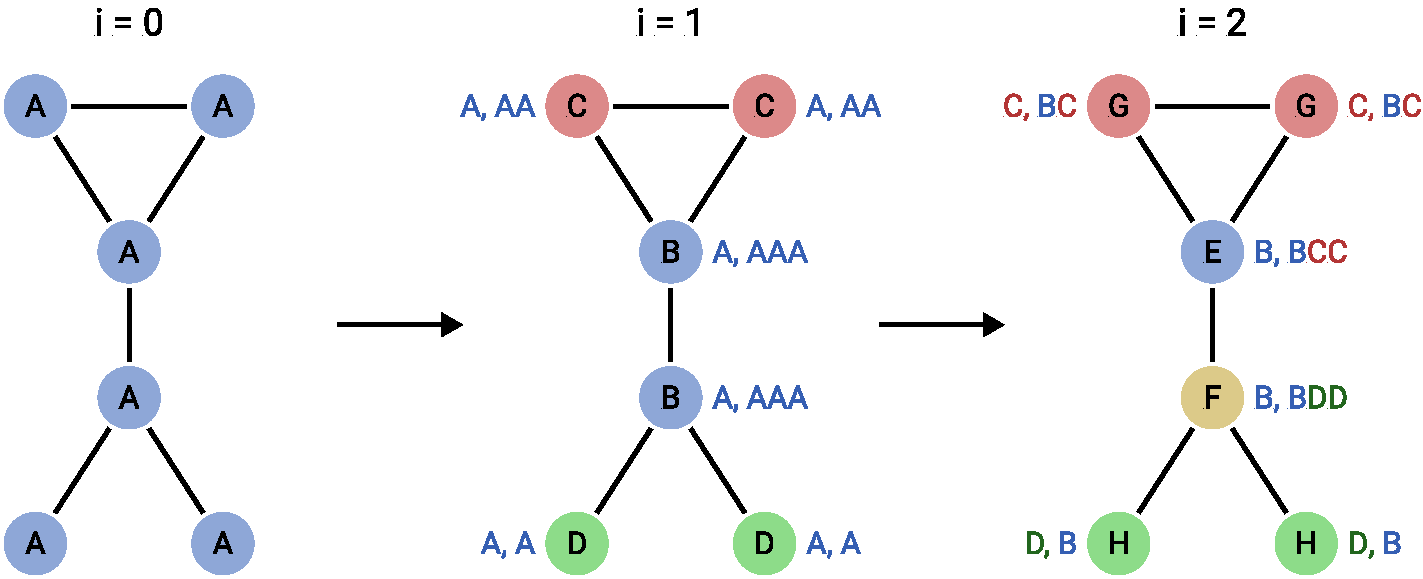
\includegraphics[width=0.75\linewidth]{gfx/related-work/wl1-refine.pdf}
	\caption[Example 1-WL color refinement steps.]{
		Example 1-WL color refinement steps.
		After two iterations the coloring stabilizes.
		Each vertex is labeled with its current color and has the aggregated neighbors, as defined in \cref{eq:related:wl1-refine}, written next to it.
	}\label{fig:related:wl1-refine}
\end{figure}

\subsubsection{The $k$-dimensional \acs{wl} algorithm}
As we just saw, the 1-\acs{wl} algorithm iteratively refines colorings of single vertices.
While the obtained colorings differ for most non-isomorphic graphs $G \not\simeq H$, 1-\acs{wl} does not generally solve the graph isomorphism problem as illustrated in \cref{fig:related:wl1-problem}.
\begin{figure}[ht]
	\centering
	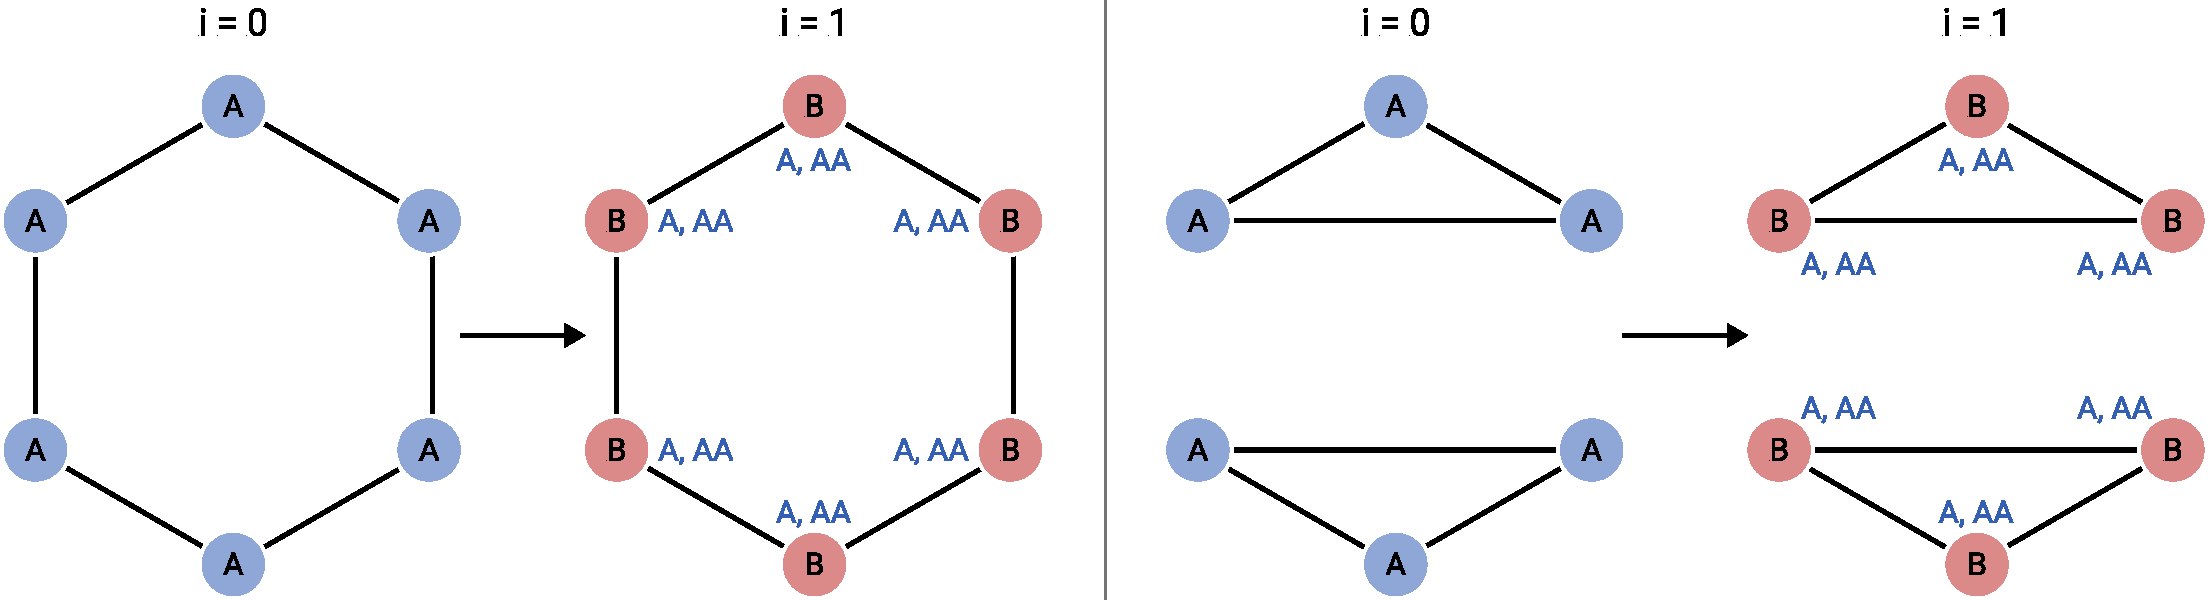
\includegraphics[width=\linewidth]{gfx/related-work/wl1-problem.pdf}
	\caption[Two simple non-isomorphic graphs that are indistinguishable by 1-\acs{wl}.]{
		Two simple non-isomorphic graphs that are indistinguishable by 1-\acs{wl}.
	}\label{fig:related:wl1-problem}
\end{figure}
By extending \ac{wl} to higher dimensions such 1-\acs{wl} indistinguishable cases can however be handled.
Analogous to the 1-dimensional definition from \cref{eq:related:wl1-refine}, the $k$-dimensional color refinement step is defined by
\begin{align}
	\chi_{G,k}^{i+1}(v) := &\ h\left(\chi_{G,k}^{i}(v), \ldblbrace (\chi_{G,k}^{i}(v[u/1]), \dots, \chi_{G,k}^{i}(v[u/k]))\, |\, u \in \mathcal{V}_G \rdblbrace\right)\label{eq:related:wlk-refine}\\
	\text{with } v = &\ (v_1, \dots, v_k) \in \mathcal{V}^k \quad\text{and}\quad v[u/j] := (v_1, \dots, v_{j-1}, u, v_{j+1}, \dots, v_k)\text{.} \nonumber
\end{align}
In 1-\acs{wl} a vertex color is refined by combining the colors of neighboring vertices.
In $k$-\acs{wl} the color of a $k$-tuple $v \in \mathcal{V}^k$ is refined by combining the colors of its neighborhood which is defined as the set of all $k$-tuples in which at most one vertex differs from $v$.
Note that each vertex $k$-tuple has one neighbor for each $u \in \mathcal{V}_G$, each of which is a $k$-tuple of vertex $k$-tuples.
This more abstract notion of neighborhood is illustrated in \cref{fig:related:wl-neighbors}.
\begin{figure}[ht]
	\centering
	\begin{subfigure}{0.33\textwidth}
		\centering
		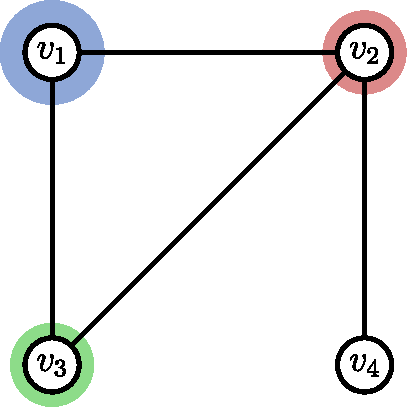
\includegraphics[width=0.8\linewidth]{gfx/related-work/wl1-neighbors.pdf}
		\subcaption{1-WL $v_1$ neighbors}\label{fig:related:wl-neighbors:1}
	\end{subfigure}%
	\begin{subfigure}{0.33\textwidth}
		\centering
		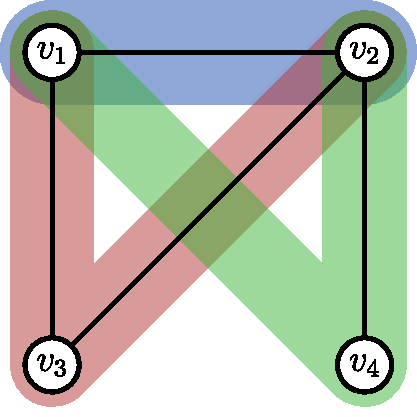
\includegraphics[width=0.8\linewidth]{gfx/related-work/wl2-neighbors.pdf}
		\subcaption{2-WL $(v_1, v_2)$ neighbors}\label{fig:related:wl-neighbors:2}
	\end{subfigure}%
	\begin{subfigure}{0.33\textwidth}
		\centering
		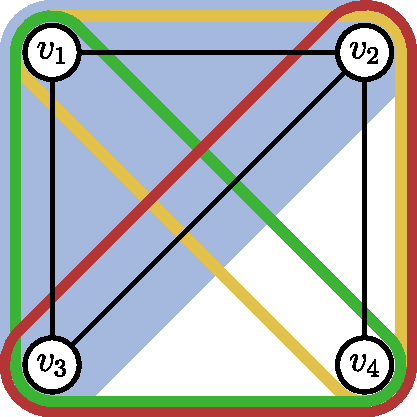
\includegraphics[width=0.8\linewidth]{gfx/related-work/wl3-neighbors.pdf}
		\subcaption{3-WL $(v_1, v_2, v_3)$ neighbors}\label{fig:related:wl-neighbors:3}
	\end{subfigure}
	\caption[\ac{wl} neighborhoods for different values of $k$.]{
		Tuple neighborhoods for different values of $k$.
		The vertices highlighted in \textcolor{t_blue}{blue} form the root tuple whose neighbors are shown.
		Each neighbor is highlighted with a different color, except for 3-WL where the \textcolor{t_red}{red}, \textcolor{t_green}{green} and \textcolor{t_darkyellow}{yellow} triples actually form the single neighbor for $u = v_4$ (see~\cref{eq:related:wlk-refine}).
	}\label{fig:related:wl-neighbors}
\end{figure}
For $k = 2$ this means that each potential edge $(v, w) \in \mathcal{V}_G^2$ has all possible paths of length $2$ from $v$ to $w$ as its neighbors (see~\cref{fig:related:wl-neighbors:2}).
Also note that, even though $k$-\acs{wl} refines $k$-tuple colors, lower-dimensional structures still get their own colors since a tuple does not have to consist of distinct vertices, i.e.\ in $k$-\acs{wl} the color of a single vertex $v \in \mathcal{V}_G$ is described by $\bar{\chi}_{G, k}(s)$ for $s = (v, \dots, v) \in \mathcal{V}_G^k$.

Let us now look at how the tuple colors are initialized.
For this we use subgraph \textit{isomorphism types} which determine the initial color $\chi_{G,k}^0(v)$ of each $k$-tuple $v$.
For $k = 1$ the isomorphism type of a vertex $v$ directly corresponds to its label $l_G(v)$.
For $k > 1$ the isomorphism types more generally correspond to the classes of isomorphic ordered subgraphs of $G$ induced by the $k$-tuples $\mathcal{V}_G^k$.
Formally this means that
\begin{align}
	\chi_{G,k}^0(v_1, \dots, v_k) = \chi_{G,k}^0(w_1, \dots, w_k) \label{eq:related:wlk-init}
	\iff &\ \forall i: l_G(v_i) = l_G(w_i) \\
	\land &\ \forall i, j: v_i = v_j \leftrightarrow w_i = w_j \nonumber \\
	\land &\ \forall i, j: (v_i, v_j) \in \mathcal{E}_G \leftrightarrow (w_i, w_j) \in \mathcal{E}_G \text{.} \nonumber
\end{align}
If no explicit vertex labeling $l_G$ is given, a single constant label for all vertices is assumed.
Also note that there is a fundamental difference in how the adjacency information encoded in $\mathcal{E}_G$ is used in 1-\acs{wl} vs.\ $k$-\acs{wl}:
In 1-\acs{wl} a vertex coloring by itself cannot encode adjacency which is why this information is explicitly incorporated in each refinement step via $\Gamma_G$ (see~\cref{eq:related:wl1-refine}).
In $k$-\acs{wl} on the other hand each pair of vertices $(v, u) \in \mathcal{V}_G^2$ appears in at least one $k$-tuple (assuming $k \geq 2$) and therefore has at least one color which can implicitly encode the adjacency information.
Edges and non-edges are colored differently in the initial coloring as defined in \cref{eq:related:wlk-init};
thus no explicit adjacency information is needed in the $k$-\acs{wl} color refinement step defined in \cref{eq:related:wlk-refine}.

\subsubsection{Discriminative Power of \acs{wl}}
Now we will look at the types of graphs that can be distinguished by \acs{wl} in relation to the \acs{wl}-dimension $k$.
\begin{thm}
	$G \mathrel{\not\simeq_k} H \implies G \mathrel{\not\simeq_{k+1}} H$, i.e.\ the discriminative power of $k$-\acs{wl} grows with $k$.
	\begin{hproof}
		All $k$-tuples can be mapped to $(k+1)$-tuples, e.g.\ via $\varphi(v_1, \dots, v_k) = (v_1, \dots, v_k, v_k)$.
	\end{hproof}
\end{thm}
\begin{figure}[ht]
	\centering
	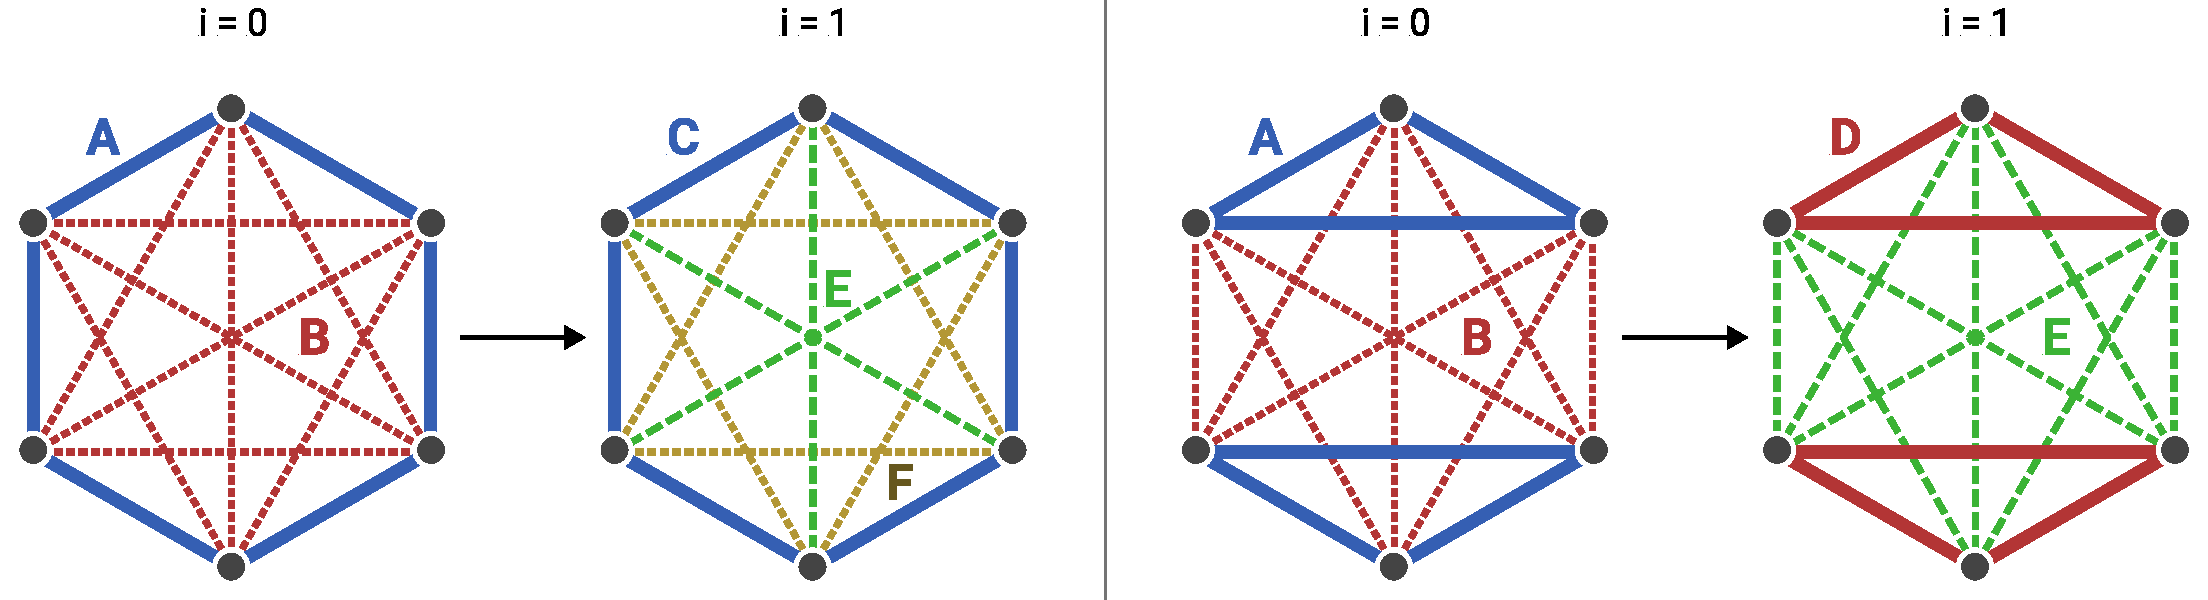
\includegraphics[width=\linewidth]{gfx/related-work/wl2-problem-solution.pdf}
	\caption[Two simple non-isomorphic graphs that are indistinguishable by 1-\acs{wl}.]{
		Two simple non-isomorphic graphs that are indistinguishable by 1-\acs{wl}.
	}\label{fig:related:wl2-problem-solution}
\end{figure}

\subsection{Spectral Graph Theory}%
\label{sec:related:character:spectral}

\section{Graph Classification and Regression}%
\label{sec:related:gcr}

The existing approaches to tackle the \ac{gcr} problem can be categorized into three main families:
\begin{enumerate*}
	\item Explicit graph embeddings,
	\item graph kernels and
	\item graph neural networks
\end{enumerate*}.
We will now look at the characteristics of those families and give a brief overview of specific methods.

\subsection{Explicit Graph Embeddings}%
\label{sec:related:gcr:embed}

The basic idea of explicit graph embedding approaches is to map a graph $G \in \mathbb{G}$ to some vector in a finite vector space $\mathcal{X} = \mathbb{R}^d$.
A function $f: \mathbb{G} \to \mathcal{X}$ is called a \textit{graph embedding function}.
By embedding a graph into $\mathcal{X}$, any classification or regression algorithm that works with vectors can then be applied to solve the \ac{gcr} problem.

The so-called vertex embedding problem is closely related to the graph embedding problem.
As the name suggests, a \textit{vertex embedding function} $f_G: V \to \mathcal{X}$ maps all vertices $v \in V$ of a graph $G$ into $\mathcal{X}$.
The embedding vector $f_G(v)$ ideally encodes relevant information about a vertex and its structural position in $G$.
It can be used to solve the vertex classification and regression problem via arbitrary \ac{ml} methods for vectors.
We will now look at two main families of explicit graph and vertex embedding approaches.

\subsubsection{Fingerprint Embeddings}

The first works on graph embeddings were motivated by the study of chemical structures~\cite{Adamson1973}\cite{Willett1986}.
There a molecule can be interpreted as a labeled graph for which the \ac{gcr} problem corresponds to the prediction of some chemical property, e.g.\ toxicity or solubility.
So-called \textit{fingerprint embeddings} try to match a fixed set of subgraphs $S_1, \dots, S_d$ to the input graph.
The embedding of a graph $G$ is a binary vector $f(G) = x \in {\{0, 1\}}^d$ with $x_i = \mathds{1}[\text{$S_i$ is subgraph of $G$}]$, where $\mathds{1}$ denotes the indicator function.
This simple approach usually requires a careful choice of subgraphs but can still be competitive with the other more recent approaches we will look at in the following sections.
Fingerprint embeddings are for example used in multiple state-of-the-art toxicity prediction tools like RASAR~\cite{Luechtefeld2018}\cite{ToxTrack}, ProTox~\cite{Drwal2014}\cite{Banerjee2018}\cite{ProTox} or the \ac{toxTest}~\cite{TEST}.

\subsubsection{Skip-gram inspired Embeddings}

Skip-gram embeddings were introduced by \citeauthor{Mikolov2013} as part of the well-known \texttt{word2vec}~\cite{Mikolov2013} word embedding method from \ac{nlp}.
While a fingerprint embedding explicitly assigns an interpretation to each embedding dimension (i.e.\ to each standard basis vector), a skip-gram embedding only optimizes the distance between embedding vectors based on the similarity of the embedded instances without providing an interpretation of the embedding dimensions.

\paragraph{word2vec}
Let us first look at the \texttt{word2vec} skip-gram method.
It gets a sequence of words $(w_0, \dots, w_n)$ as input and outputs embedding vectors $f(w_0), \dots, f(w_n) \in \mathbb{R}^d$.
To do this the context $C_k(w_i) = \{ w_{i-k}, \dots, w_{i + k} \}$ is computed for all words where $w_i$ is the so-called \textit{context root}.
The word contexts are then used to optimize the following log-likelihood objective:
\begin{gather}
	\max_{f, f_C} \sum_{i = 1}^n \log P(C_k(w_i) | w_i)\ =\ \max_{f, f_C} \sum_{i = 1}^n \smashoperator[r]{\sum_{w_j \in C_k(w_i)}}\, \left[ {f(w_i)}^\top f_C(w_j) - \log Z_{w_i} \right] \label{eq:related:gcr:embed:word2vec}\\
	\text{with } P(C_k(w_i) | w_i) := \prod_{\mathclap{w_j \in C_k(w_i)}}\, \overbrace{\frac{\exp\left({f(w_i)}^\top f_C(w_j)\right)}{Z_{w_i}}}^{P(w_j | w_i)}
	\text{ and } Z_{w_i} := \sum_{j = 1}^n \exp\left({f(w_i)}^\top f_C(w_j)\right) \nonumber
\end{gather}
\texttt{word2vec} essentially uses an expectation maximization scheme to maximize the probabilities $P(w_j | w_i)$ of observing the context words $w_j \in C_k(w_i)$ of all words $w_i$.
Those probabilities are described by the overlap of the embeddings $f(w_i)$ of words $w_i$ and the embeddings $f_C(w_j)$ of their context words $w_j$.
Intuitively this means that words with similar contexts will be mapped close to each other in the embedding space.
Note that \texttt{word2vec} actually finds two embeddings $f(w)$ and $f_C(w)$ for each word of which only the first is returned.
The two embeddings represent two different perspectives on words: $f$ describes a word $w_i$ as the root of a context $C_k(w_i)$, $f_C$ on the other hand describes a word $w_j$ as part of a context $C_k(w_i) \ni w_j$.

\paragraph{Vertex Embeddings}
Skip-gram embeddings can be  na{\"\i}vely extended to graphs by realizing that \texttt{word2vec} effectively already is a vertex embedding method for linear graphs in which $C_k(v)$ is simply the $k$-neighborhood of the vertex/word $v$.
The problem with this na{\"\i}ve extension is that the sizes of $k$-neighborhoods in arbitrary graphs can be much larger and often tend to grow exponentially with $k$.
To deal with this computational problem the so-called DeepWalk~\cite{Perozzi2014} and \texttt{node2vec}~\cite{Grover2016} methods perform random walks of fixed length to effectively take samples from the neighborhood of vertices.
Both methods only differ in the transition matrix that is used for the random walk.
Another difference of DeepWalk and \texttt{node2vec} compared to \texttt{word2vec} is the so-called \textit{feature space symmetry} which states that the context root interpretation ($f$) of a vertex should be symmetric to its context element interpretation ($f_C$), i.e.\ $f = f_C$.
The combination of random walk context sampling and and the feature space symmetry assumption can be used to compute vertex embeddings even for very large graphs.

\paragraph{Graph Embeddings}
Skip-gram methods can not only be used for vertex embeddings but also to embed entire graphs.
One way to do this is via the \texttt{graph2vec}~\cite{Narayanan2017} method.
It is inspired by \texttt{doc2vec}~\cite{Le2014} which in turn is based on \texttt{word2vec}.
\texttt{graph2vec} gets a set of graphs $\mathbb{G} = \{ G_1, \dots G_N \}$ as input and outputs graph embeddings $f(G_1), \dots, f(G_N)$.
While in \texttt{word2vec} every word can be a context root as well as a context element, \texttt{graph2vec} uses the graphs $\mathbb{G}$ as context roots.
The context $C_k(G_i)$ of a graph $G_i = (\mathcal{V}_i, \mathcal{E}_i)$ is defined as
\begin{equation}
	C_k(G_i) := \bigcup_{\mathclap{v_j \in \mathcal{V}_i}}\, {\left\{ {\textrm{WL}_l(G_i)}_j \right\}}_{l = 0}^k % chktex 21
	\text{ with } \textrm{WL}_l(G) := \text{$l$ iter.\ \acs{wl}-1 coloring of $G$.}
\end{equation}
Intuitively this context can be understood as the set of \acs{wl}-distinguishable subgraphs of $G_i$ with diameter $\leq 2k$.
Since \ac{wl} is used to identify distinct subgraphs, \texttt{graph2vec} can only be applied to graphs with discrete vertex labels.
Using the previous definitions, the context root embedding function has the signature $f: \mathbb{G} \to \mathbb{R}^d$ while the context element embedding function is of type $f_C: \bigcup_{G_i \in \mathbb{G}} C_k(G_i) \to \mathbb{R}^d$.
To find those embeddings the \texttt{word2vec} objective from \cref{eq:related:gcr:embed:word2vec} is reused.
Analogous to \texttt{word2vec}, \texttt{graph2vec} therefore embeds graphs that share subgraphs close to each other, whereas graphs that do not share substructures tend to be embedded further away from each other.

\subsection{Graph Kernels}%
\label{sec:related:gcr:kernel}

Instead of explicitly mapping a graph or vertices into a vector space, one can also do so implicitly by employing the kernel trick.
There is a large variety of so-called \acp{gk} to do this.
\acp{gk} can be used in combination with any kernel method, typically a \ac{svm}, to solve the \ac{gcr} problem.
While there is a large variety of different \acp{gk}, we will focus on those that are based on the previously described family of \ac{wl} algorithms.

\paragraph{\ac{wl} subtree kernel}

\paragraph{\ac{wl} shortest path kernel}

\paragraph{Higher dimensional \ac{wl} kernels}

\subsection{Graph Neural Networks}%
\label{sec:related:gcr:nn}

\subsubsection{Spatial GNNs}

\subsubsection{Spectral GNNs}
